% Options for packages loaded elsewhere
\PassOptionsToPackage{unicode}{hyperref}
\PassOptionsToPackage{hyphens}{url}
%
\documentclass[
  french,
  ignorenonframetext,
]{beamer}
\usepackage{pgfpages}
\setbeamertemplate{caption}[numbered]
\setbeamertemplate{caption label separator}{: }
\setbeamercolor{caption name}{fg=normal text.fg}
\beamertemplatenavigationsymbolsempty
% Prevent slide breaks in the middle of a paragraph
\widowpenalties 1 10000
\raggedbottom
\setbeamertemplate{part page}{
  \centering
  \begin{beamercolorbox}[sep=16pt,center]{part title}
    \usebeamerfont{part title}\insertpart\par
  \end{beamercolorbox}
}
\setbeamertemplate{section page}{
  \centering
  \begin{beamercolorbox}[sep=12pt,center]{part title}
    \usebeamerfont{section title}\insertsection\par
  \end{beamercolorbox}
}
\setbeamertemplate{subsection page}{
  \centering
  \begin{beamercolorbox}[sep=8pt,center]{part title}
    \usebeamerfont{subsection title}\insertsubsection\par
  \end{beamercolorbox}
}
\AtBeginPart{
  \frame{\partpage}
}
\AtBeginSection{
  \ifbibliography
  \else
    \frame{\sectionpage}
  \fi
}
\AtBeginSubsection{
  \frame{\subsectionpage}
}
\usepackage{lmodern}
\usepackage{amssymb,amsmath}
\usepackage{ifxetex,ifluatex}
\ifnum 0\ifxetex 1\fi\ifluatex 1\fi=0 % if pdftex
  \usepackage[T1]{fontenc}
  \usepackage[utf8]{inputenc}
  \usepackage{textcomp} % provide euro and other symbols
\else % if luatex or xetex
  \usepackage{unicode-math}
  \defaultfontfeatures{Scale=MatchLowercase}
  \defaultfontfeatures[\rmfamily]{Ligatures=TeX,Scale=1}
\fi
% Use upquote if available, for straight quotes in verbatim environments
\IfFileExists{upquote.sty}{\usepackage{upquote}}{}
\IfFileExists{microtype.sty}{% use microtype if available
  \usepackage[]{microtype}
  \UseMicrotypeSet[protrusion]{basicmath} % disable protrusion for tt fonts
}{}
\makeatletter
\@ifundefined{KOMAClassName}{% if non-KOMA class
  \IfFileExists{parskip.sty}{%
    \usepackage{parskip}
  }{% else
    \setlength{\parindent}{0pt}
    \setlength{\parskip}{6pt plus 2pt minus 1pt}}
}{% if KOMA class
  \KOMAoptions{parskip=half}}
\makeatother
\usepackage{xcolor}
\IfFileExists{xurl.sty}{\usepackage{xurl}}{} % add URL line breaks if available
\IfFileExists{bookmark.sty}{\usepackage{bookmark}}{\usepackage{hyperref}}
\hypersetup{
  pdftitle={Alba Marina Málaga Sabogal},
  pdfauthor={Audition pour le poste de maître de conférences n°4730},
  pdflang={fr},
  hidelinks,
  pdfcreator={LaTeX via pandoc}}
\urlstyle{same} % disable monospaced font for URLs
\newif\ifbibliography
\usepackage{longtable,booktabs}
\usepackage{caption}
% Make caption package work with longtable
\makeatletter
\def\fnum@table{\tablename~\thetable}
\makeatother
\usepackage{graphicx}
\makeatletter
\def\maxwidth{\ifdim\Gin@nat@width>\linewidth\linewidth\else\Gin@nat@width\fi}
\def\maxheight{\ifdim\Gin@nat@height>\textheight\textheight\else\Gin@nat@height\fi}
\makeatother
% Scale images if necessary, so that they will not overflow the page
% margins by default, and it is still possible to overwrite the defaults
% using explicit options in \includegraphics[width, height, ...]{}
\setkeys{Gin}{width=\maxwidth,height=\maxheight,keepaspectratio}
% Set default figure placement to htbp
\makeatletter
\def\fps@figure{htbp}
\makeatother
\setlength{\emergencystretch}{3em} % prevent overfull lines
\providecommand{\tightlist}{%
  \setlength{\itemsep}{0pt}\setlength{\parskip}{0pt}}
\setcounter{secnumdepth}{-\maxdimen} % remove section numbering
\ifxetex
  % Load polyglossia as late as possible: uses bidi with RTL langages (e.g. Hebrew, Arabic)
  \usepackage{polyglossia}
  \setmainlanguage[]{french}
\else
  \usepackage[shorthands=off,main=french]{babel}
\fi

\title{Alba Marina Málaga Sabogal}
\author{Audition pour le poste de maître de conférences n°4730}
\date{25 mai 2020}

\begin{document}
\frame{\titlepage}

\hypertarget{parcours}{%
\section{Parcours}\label{parcours}}

\begin{frame}{Études et vie professionnelle}
\protect\hypertarget{uxe9tudes-et-vie-professionnelle}{}
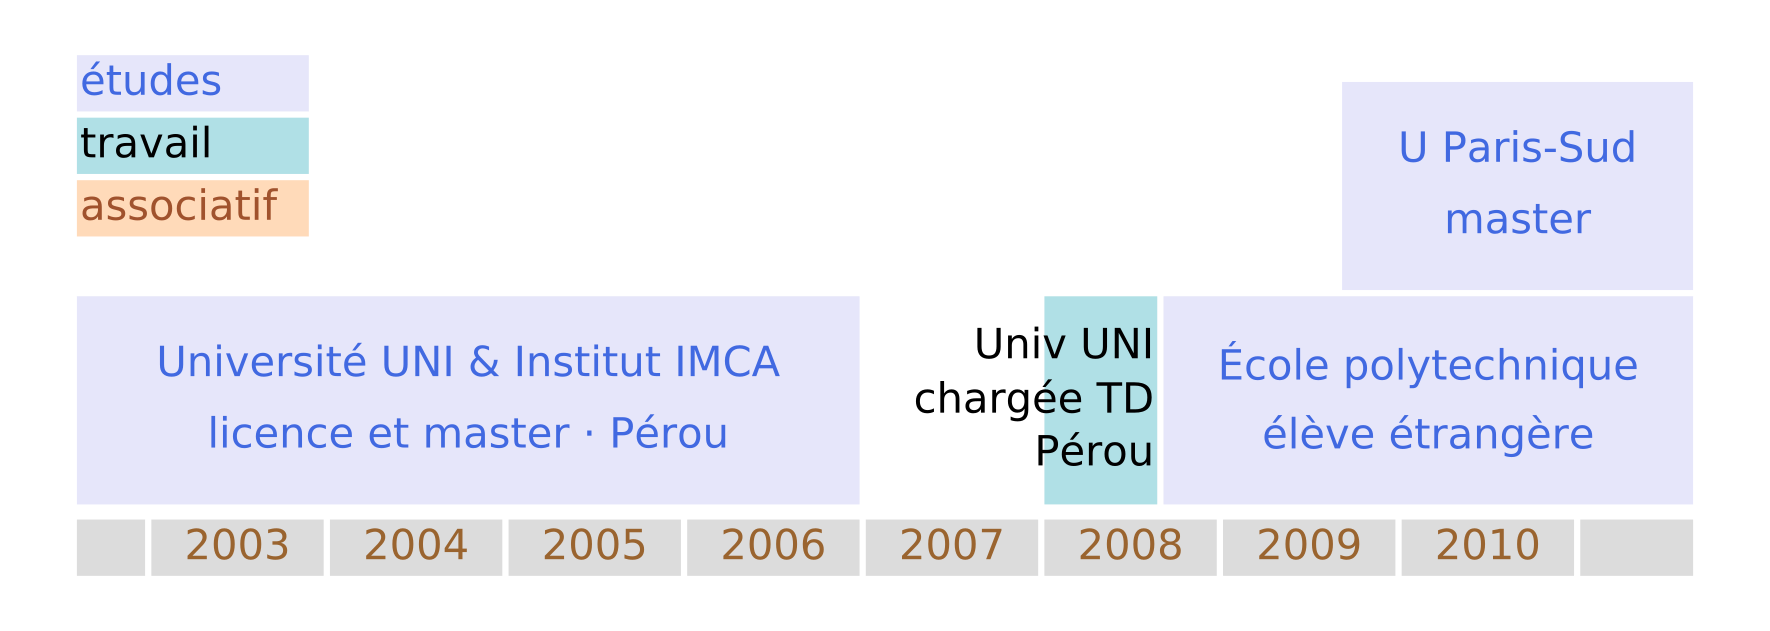
\includegraphics[width=0.9\textwidth,height=\textheight]{img/alba-timeline-etudes.png}

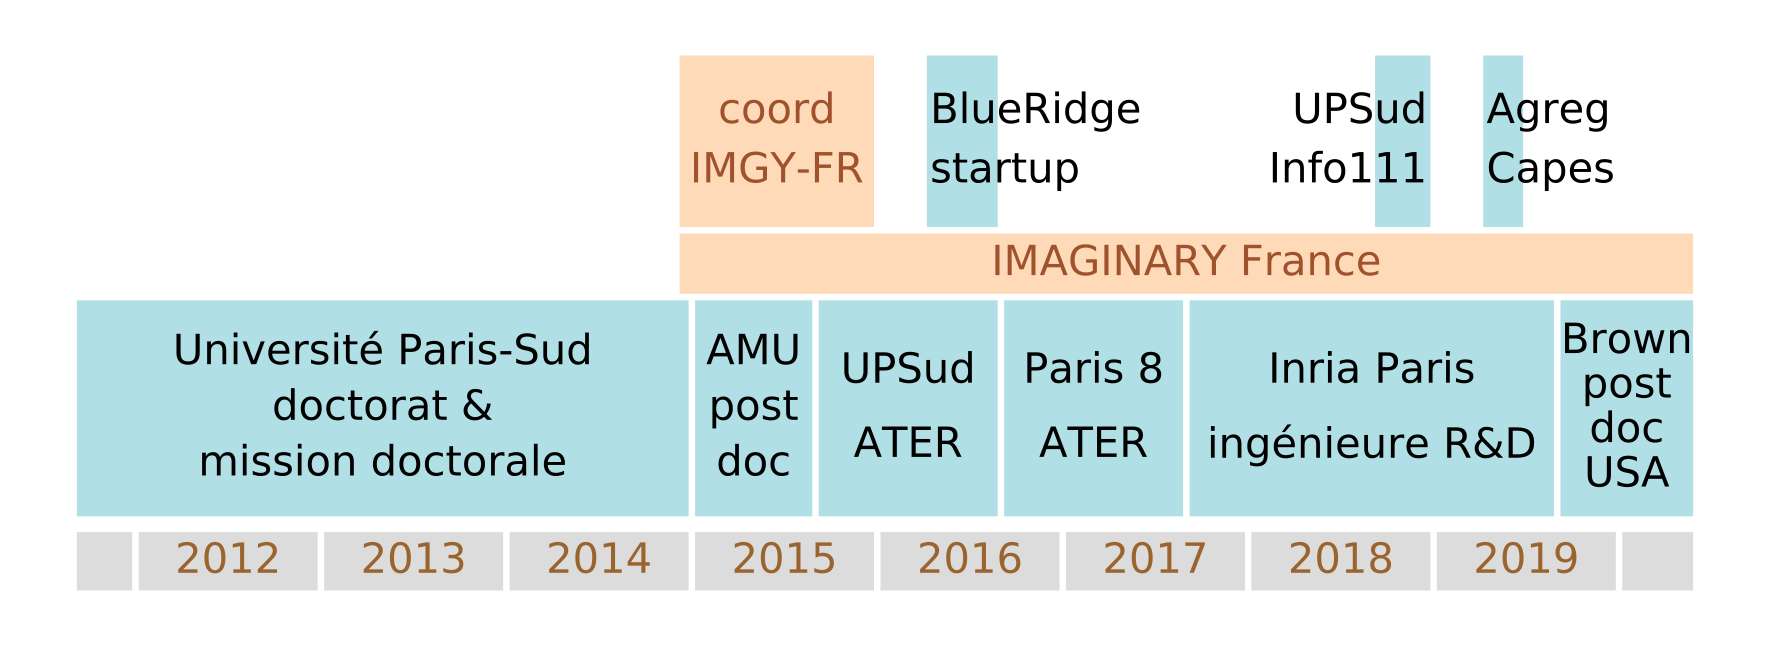
\includegraphics[width=0.9\textwidth,height=\textheight]{img/alba-timeline-viepro.png}
\end{frame}

\hypertarget{recherche}{%
\section{Recherche}\label{recherche}}

\begin{frame}{Mes mentors au fil du temps}
\protect\hypertarget{mes-mentors-au-fil-du-temps}{}
En projet et stage de 2e et 3e années à l'École polytechnique,\\
en M2 puis en thèse à Orsay, puis en postdoc à Marseille\\
et à Providence aux États-Unis, j'ai été encadrée par:

\begin{longtable}[]{@{}lll@{}}
\toprule
\endhead
2010--2011 & Projet scientifique collectif & Gilles
Courtois\tabularnewline
2011 & Stage de recherche & Vadim Lyubashevsky\tabularnewline
2011 & Stage de recherche M2 & Sylvie Ruette\tabularnewline
2011--2014 & Thèse doctorale & Jean-Christophe Yoccoz\tabularnewline
2015 & Post-doctorat & Alexander Bufetov\tabularnewline
2019--2020 & Post-doctorat & Richard Schwartz\tabularnewline
\bottomrule
\end{longtable}

Depuis 2015 j'ai une collaboration suivie avec Serge Troubetzkoy sur la
dynamique de surfaces de translation de mesure infinie.
\end{frame}

\begin{frame}{Les systèmes dynamiques}
\protect\hypertarget{les-systuxe8mes-dynamiques}{}
\begin{itemize}
\tightlist
\item
  Évolution déterministe à court terme, connue
\item
  Questions concernant l'évolution à long terme
\end{itemize}

\begin{block}{Exemple: les rotations du cercle}
\protect\hypertarget{exemple-les-rotations-du-cercle}{}
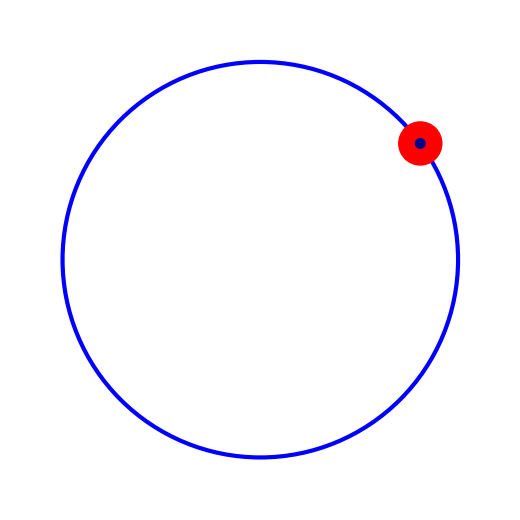
\includegraphics[width=0.6\textwidth,height=\textheight]{img/itere_00.png}
\end{block}
\end{frame}

\begin{frame}{Les systèmes dynamiques}
\protect\hypertarget{les-systuxe8mes-dynamiques-1}{}
\begin{itemize}
\tightlist
\item
  Évolution déterministe à court terme, connue
\item
  Questions concernant l'évolution à long terme
\end{itemize}

\begin{block}{Exemple: les rotations du cercle}
\protect\hypertarget{exemple-les-rotations-du-cercle-1}{}
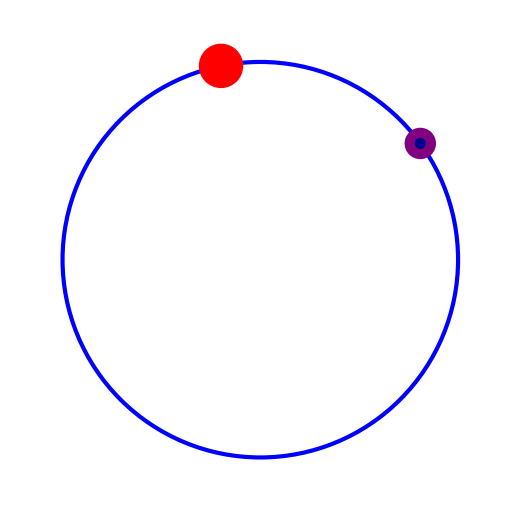
\includegraphics[width=0.6\textwidth,height=\textheight]{img/itere_01.png}
\end{block}
\end{frame}

\begin{frame}{Les systèmes dynamiques}
\protect\hypertarget{les-systuxe8mes-dynamiques-2}{}
\begin{itemize}
\tightlist
\item
  Évolution déterministe à court terme, connue
\item
  Questions concernant l'évolution à long terme
\end{itemize}

\begin{block}{Exemple: les rotations du cercle}
\protect\hypertarget{exemple-les-rotations-du-cercle-2}{}
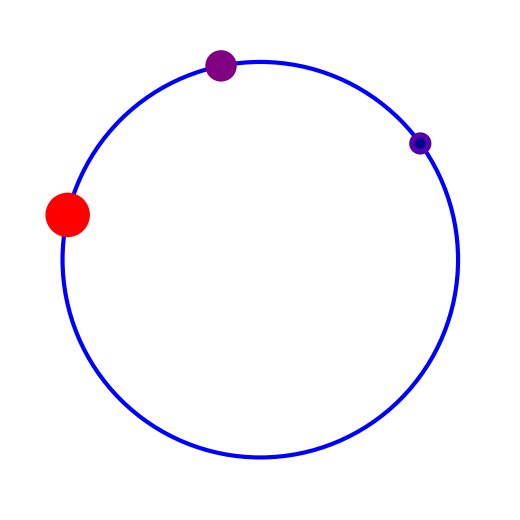
\includegraphics[width=0.6\textwidth,height=\textheight]{img/itere_02.png}
\end{block}
\end{frame}

\begin{frame}{Les systèmes dynamiques}
\protect\hypertarget{les-systuxe8mes-dynamiques-3}{}
\begin{itemize}
\tightlist
\item
  Évolution déterministe à court terme, connue
\item
  Questions concernant l'évolution à long terme
\end{itemize}

\begin{block}{Exemple: les rotations du cercle}
\protect\hypertarget{exemple-les-rotations-du-cercle-3}{}
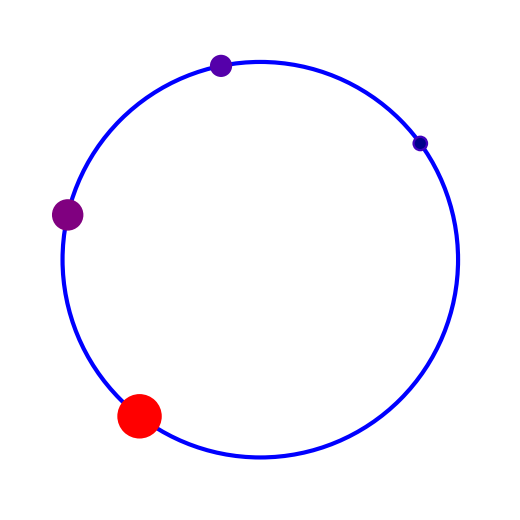
\includegraphics[width=0.6\textwidth,height=\textheight]{img/itere_03.png}
\end{block}
\end{frame}

\begin{frame}{Les systèmes dynamiques}
\protect\hypertarget{les-systuxe8mes-dynamiques-4}{}
\begin{itemize}
\tightlist
\item
  Évolution déterministe à court terme, connue
\item
  Questions concernant l'évolution à long terme
\end{itemize}

\begin{block}{Exemple: les rotations du cercle}
\protect\hypertarget{exemple-les-rotations-du-cercle-4}{}
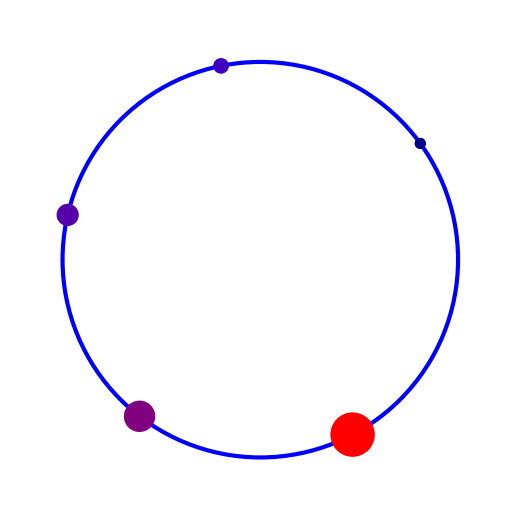
\includegraphics[width=0.6\textwidth,height=\textheight]{img/itere_04.png}
\end{block}
\end{frame}

\begin{frame}{Les systèmes dynamiques}
\protect\hypertarget{les-systuxe8mes-dynamiques-5}{}
\begin{itemize}
\tightlist
\item
  Évolution déterministe à court terme, connue
\item
  Questions concernant l'évolution à long terme
\end{itemize}

\begin{block}{Exemple: les rotations du cercle}
\protect\hypertarget{exemple-les-rotations-du-cercle-5}{}
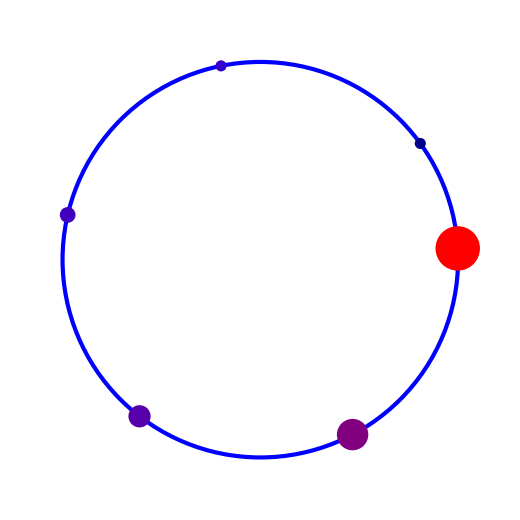
\includegraphics[width=0.6\textwidth,height=\textheight]{img/itere_05.png}
\end{block}
\end{frame}

\begin{frame}{Les systèmes dynamiques}
\protect\hypertarget{les-systuxe8mes-dynamiques-6}{}
\begin{itemize}
\tightlist
\item
  Évolution déterministe à court terme, connue
\item
  Questions concernant l'évolution à long terme
\end{itemize}

\begin{block}{Exemple: les rotations du cercle}
\protect\hypertarget{exemple-les-rotations-du-cercle-6}{}
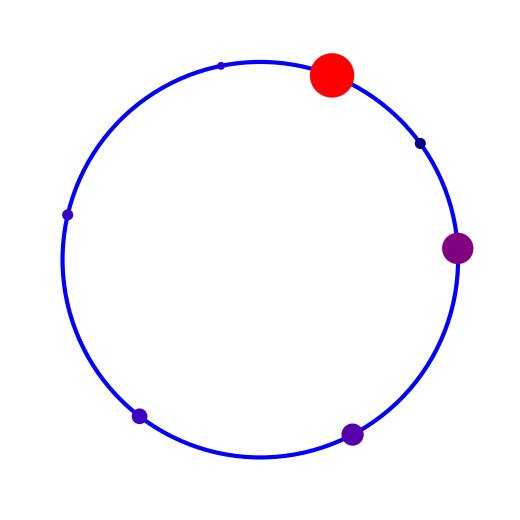
\includegraphics[width=0.6\textwidth,height=\textheight]{img/itere_06.png}
\end{block}
\end{frame}

\begin{frame}{Les systèmes dynamiques}
\protect\hypertarget{les-systuxe8mes-dynamiques-7}{}
\begin{itemize}
\tightlist
\item
  Évolution déterministe à court terme, connue
\item
  Questions concernant l'évolution à long terme
\end{itemize}

\begin{block}{Exemple: les rotations du cercle}
\protect\hypertarget{exemple-les-rotations-du-cercle-7}{}
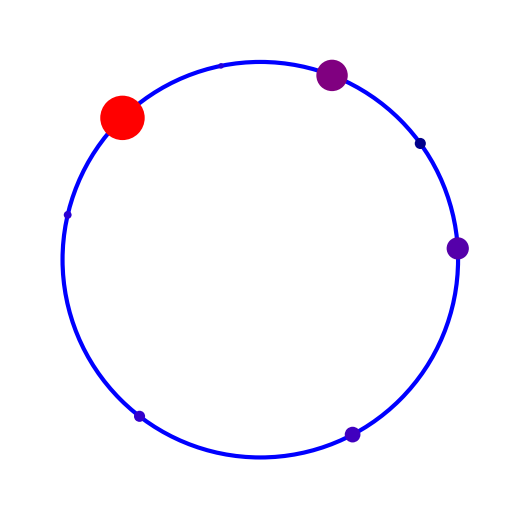
\includegraphics[width=0.6\textwidth,height=\textheight]{img/itere_07.png}
\end{block}
\end{frame}

\begin{frame}{Les systèmes dynamiques}
\protect\hypertarget{les-systuxe8mes-dynamiques-8}{}
\begin{itemize}
\tightlist
\item
  Évolution déterministe à court terme, connue
\item
  Questions concernant l'évolution à long terme
\end{itemize}

\begin{block}{Exemple: les rotations du cercle}
\protect\hypertarget{exemple-les-rotations-du-cercle-8}{}
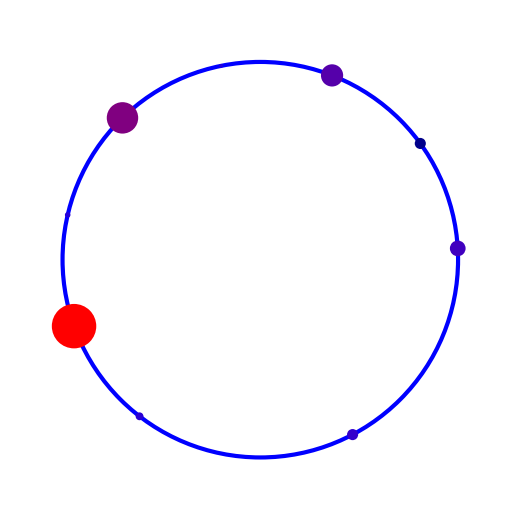
\includegraphics[width=0.6\textwidth,height=\textheight]{img/itere_08.png}
\end{block}
\end{frame}

\begin{frame}{Les systèmes dynamiques}
\protect\hypertarget{les-systuxe8mes-dynamiques-9}{}
\begin{itemize}
\tightlist
\item
  Évolution déterministe à court terme, connue
\item
  Questions concernant l'évolution à long terme
\end{itemize}

\begin{block}{Exemple: les rotations du cercle}
\protect\hypertarget{exemple-les-rotations-du-cercle-9}{}
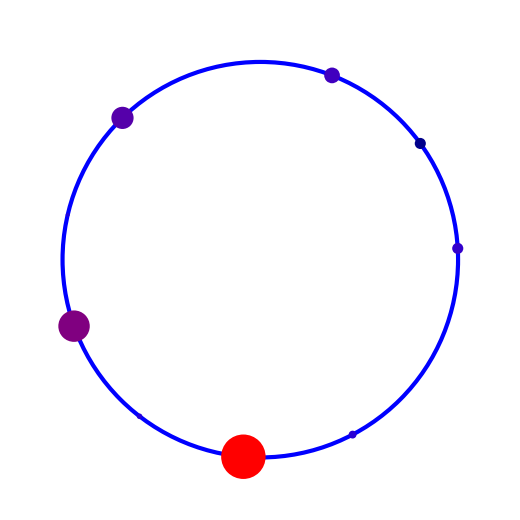
\includegraphics[width=0.6\textwidth,height=\textheight]{img/itere_09.png}
\end{block}
\end{frame}

\begin{frame}{Les systèmes dynamiques}
\protect\hypertarget{les-systuxe8mes-dynamiques-10}{}
\begin{itemize}
\tightlist
\item
  Évolution déterministe à court terme, connue
\item
  Questions concernant l'évolution à long terme
\end{itemize}

\begin{block}{Exemple: les rotations du cercle}
\protect\hypertarget{exemple-les-rotations-du-cercle-10}{}
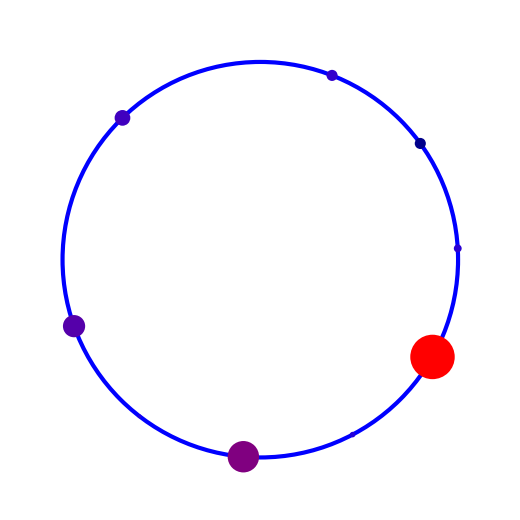
\includegraphics[width=0.6\textwidth,height=\textheight]{img/itere_10.png}
\end{block}
\end{frame}

\begin{frame}{Les systèmes dynamiques}
\protect\hypertarget{les-systuxe8mes-dynamiques-11}{}
\begin{itemize}
\tightlist
\item
  Évolution déterministe à court terme, connue
\item
  Questions concernant l'évolution à long terme
\end{itemize}

\begin{block}{Exemple: les rotations du cercle}
\protect\hypertarget{exemple-les-rotations-du-cercle-11}{}
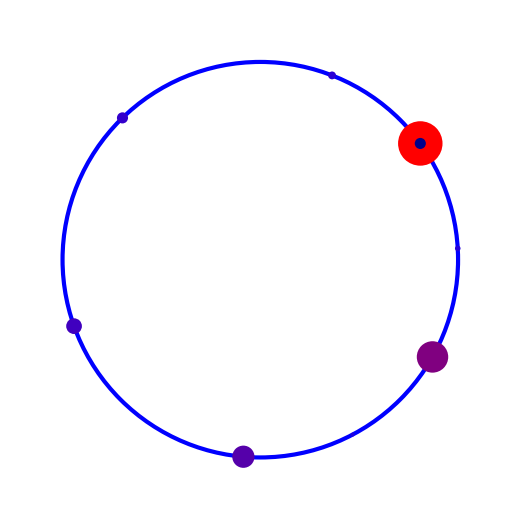
\includegraphics[width=0.6\textwidth,height=\textheight]{img/itere_11.png}
\end{block}
\end{frame}

\begin{frame}{Les systèmes dynamiques}
\protect\hypertarget{les-systuxe8mes-dynamiques-12}{}
\begin{itemize}
\tightlist
\item
  Évolution déterministe à court terme, connue
\item
  Questions concernant l'évolution à long terme
\end{itemize}

\begin{block}{Exemple: les rotations du cercle}
\protect\hypertarget{exemple-les-rotations-du-cercle-12}{}
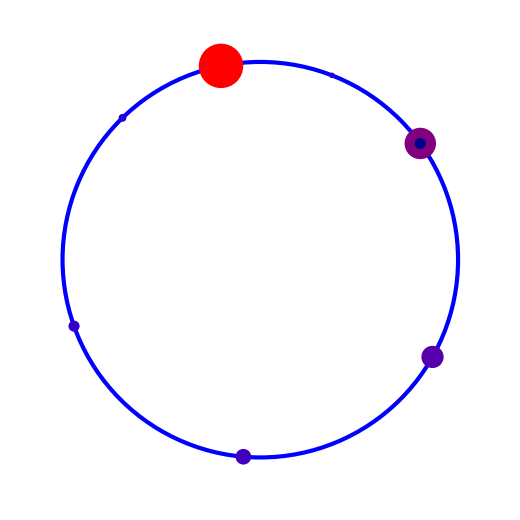
\includegraphics[width=0.6\textwidth,height=\textheight]{img/itere_12.png}
\end{block}
\end{frame}

\begin{frame}{Les systèmes dynamiques}
\protect\hypertarget{les-systuxe8mes-dynamiques-13}{}
\begin{itemize}
\tightlist
\item
  Évolution déterministe à court terme, connue
\item
  Questions concernant l'évolution à long terme
\end{itemize}

\begin{block}{Exemple: les rotations du cercle}
\protect\hypertarget{exemple-les-rotations-du-cercle-13}{}
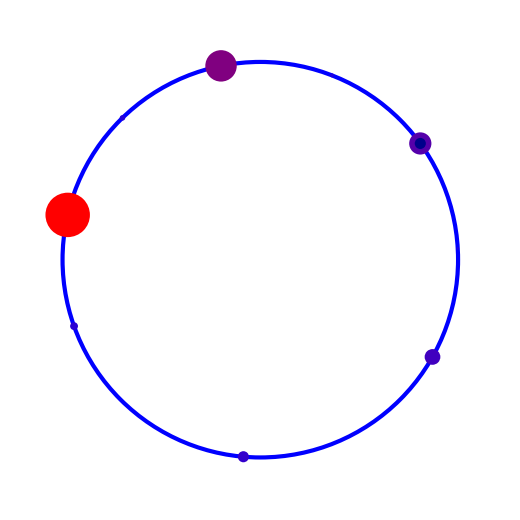
\includegraphics[width=0.6\textwidth,height=\textheight]{img/itere_13.png}
\end{block}
\end{frame}

\begin{frame}{Les systèmes dynamiques}
\protect\hypertarget{les-systuxe8mes-dynamiques-14}{}
\begin{itemize}
\tightlist
\item
  Évolution déterministe à court terme, connue
\item
  Questions concernant l'évolution à long terme
\end{itemize}

\begin{block}{Exemple: les rotations du cercle}
\protect\hypertarget{exemple-les-rotations-du-cercle-14}{}
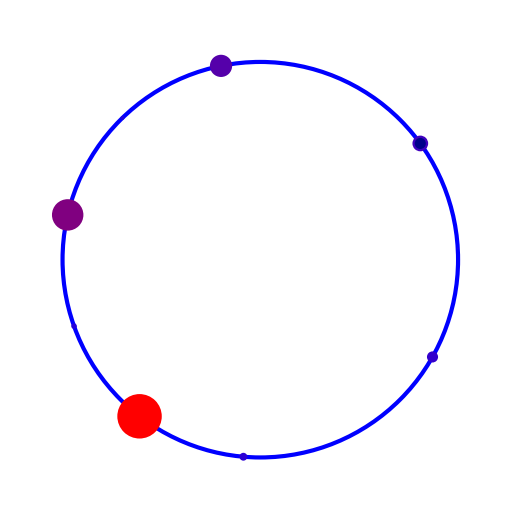
\includegraphics[width=0.6\textwidth,height=\textheight]{img/itere_14.png}
\end{block}
\end{frame}

\begin{frame}{Les systèmes dynamiques}
\protect\hypertarget{les-systuxe8mes-dynamiques-15}{}
\begin{itemize}
\tightlist
\item
  Évolution déterministe à court terme, connue
\item
  Questions concernant l'évolution à long terme
\end{itemize}

\begin{block}{Exemple: les rotations du cercle}
\protect\hypertarget{exemple-les-rotations-du-cercle-15}{}
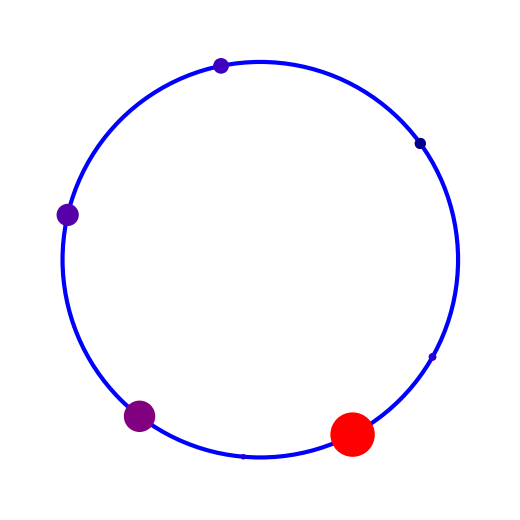
\includegraphics[width=0.6\textwidth,height=\textheight]{img/itere_15.png}
\end{block}
\end{frame}

\begin{frame}{Les systèmes dynamiques}
\protect\hypertarget{les-systuxe8mes-dynamiques-16}{}
\begin{itemize}
\tightlist
\item
  Évolution déterministe à court terme, connue
\item
  Questions concernant l'évolution à long terme
\end{itemize}

\begin{block}{Exemple: les rotations du cercle}
\protect\hypertarget{exemple-les-rotations-du-cercle-16}{}
Vue de plusieurs itérations.

\begin{figure}
\centering
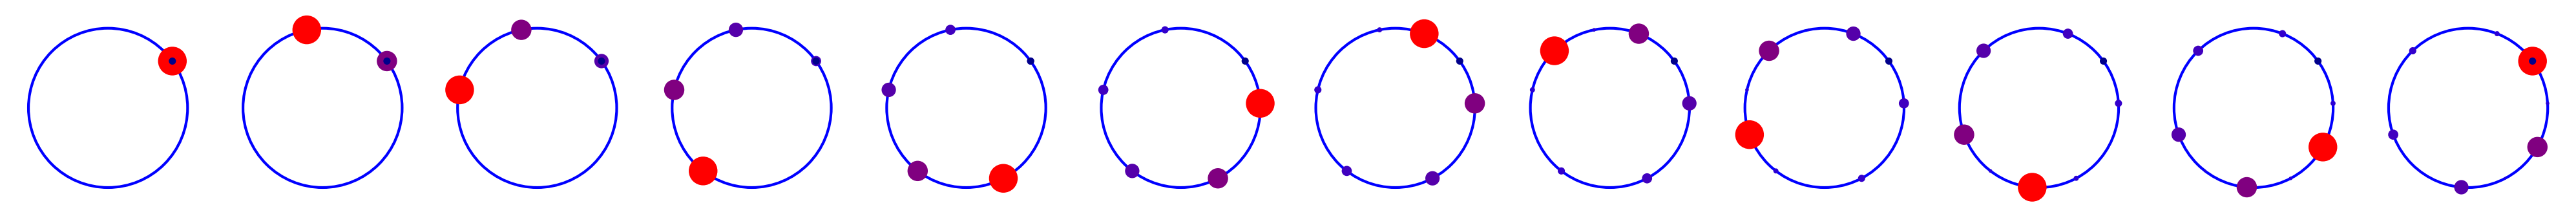
\includegraphics[width=1\textwidth,height=\textheight]{img/iteres.png}
\caption{Trajectoire d'un point par une rotation de \(\frac{2}{11}\) de
tour}
\end{figure}

\vspace{30mm}

\textbf{Thm} (Poincaré) Une rotation du cercle est périodique si et
seulement si elle est rationnelle. Sinon, elle est ergodique.
\end{block}
\end{frame}

\begin{frame}{Exemple: le flot linéaire sur un tore plat}
\protect\hypertarget{exemple-le-flot-linuxe9aire-sur-un-tore-plat}{}
\begin{block}{Qu'est-ce qu'un tore?}
\protect\hypertarget{quest-ce-quun-tore}{}
\begin{figure}
\centering
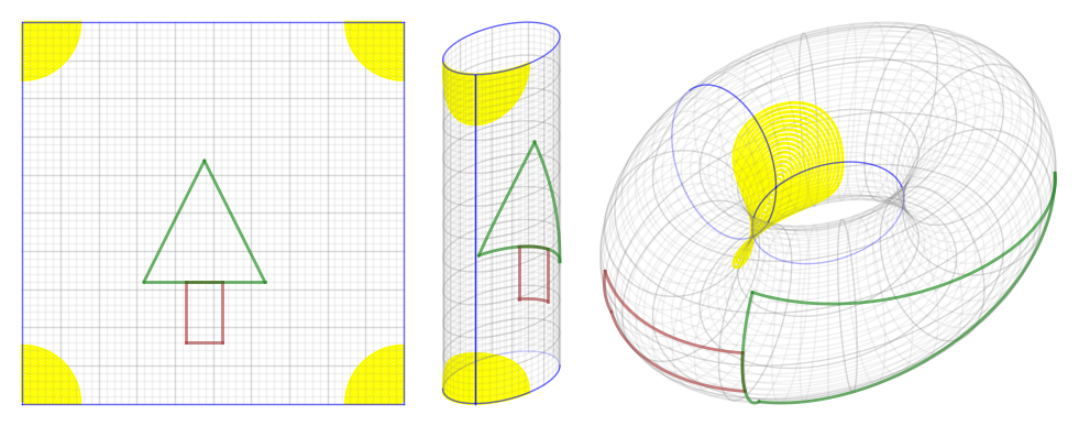
\includegraphics[width=1\textwidth,height=\textheight]{img/tore-lelievre-goujard.png}
\caption{Dessins pour comprendre le tore plat par Lelièvre et Goujard}
\end{figure}
\end{block}
\end{frame}

\begin{frame}
\begin{block}{Quelques exemples de tores}
\protect\hypertarget{quelques-exemples-de-tores}{}
\begin{figure}
\centering
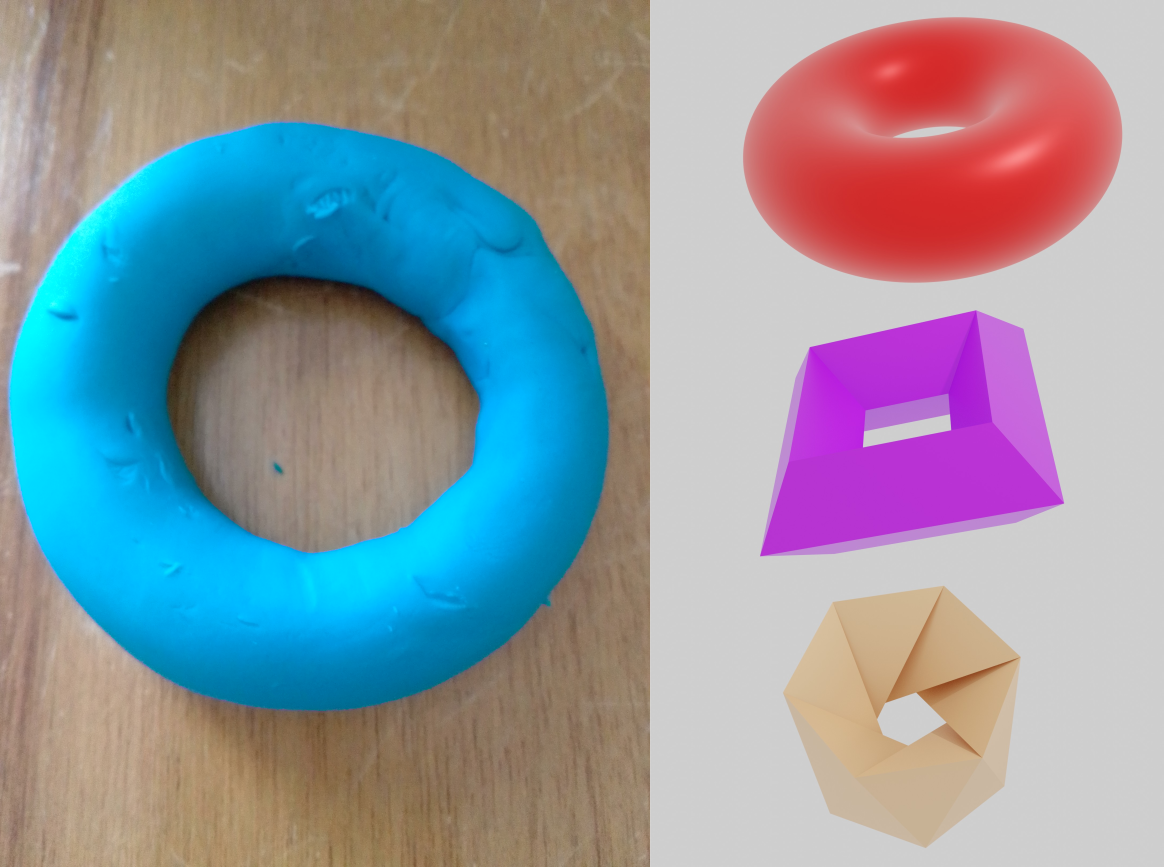
\includegraphics[width=0.8\textwidth,height=\textheight]{img/quatre-tores.png}
\caption{Tores topologiques}
\end{figure}
\end{block}
\end{frame}

\begin{frame}
\begin{block}{Comment se déplace-t-on sur un tore plat?}
\protect\hypertarget{comment-se-duxe9place-t-on-sur-un-tore-plat}{}
\vfill

\begin{figure}
\centering
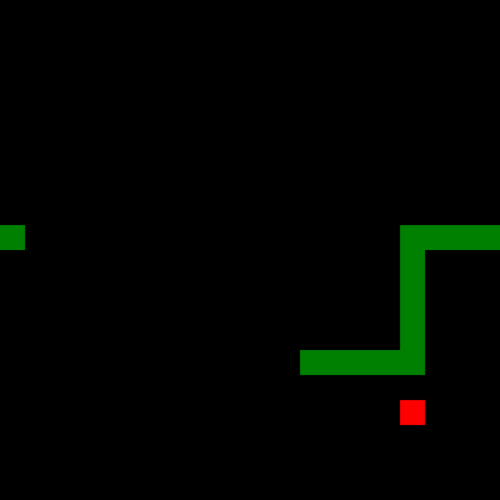
\includegraphics[width=0.6\textwidth,height=\textheight]{img/snake-on-a-torus.png}
\caption{\href{http://albamath.com/snake}{Jeu du serpent sur un tore},
par Primož Žnidar}
\end{figure}
\end{block}
\end{frame}

\begin{frame}
\begin{block}{Retour aux rotations du cercle}
\protect\hypertarget{retour-aux-rotations-du-cercle}{}
\vfill

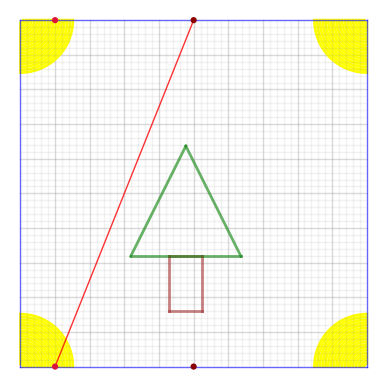
\includegraphics[width=0.35\textwidth,height=\textheight]{img/carre_traj.png}
\({}\) \({}\) \({}\)
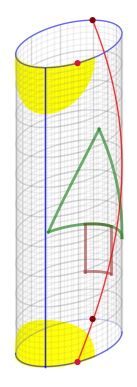
\includegraphics[width=0.15\textwidth,height=\textheight]{img/cylindre_traj.png}
\({}\) \({}\) \({}\)
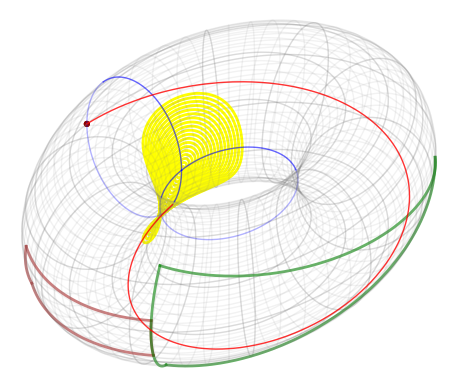
\includegraphics[width=0.4\textwidth,height=\textheight]{img/tore_traj.png}

\begin{figure}[!h]
\caption{Trajectoire sur le tore, par Lelièvre et Goujard.}
\end{figure}
\end{block}
\end{frame}

\begin{frame}{Exemple: les billards}
\protect\hypertarget{exemple-les-billards}{}
\begin{figure}
\centering
\includegraphics[width=1\textwidth,height=\textheight]{img/ball-rolling-on-a-billiard-table-hale.gif}
\caption{Départ d'une trajectoire de billard sur une table
rectangulaire.}
\end{figure}

\href{movies/ball-rolling-on-a-billiard-table-hale.mov}{Extrait} du film
«Secrets of the Surface» de Csicsery, comme les autres images et
animations de Andrea Hale à suivre.
\end{frame}

\begin{frame}{Le dépliage des billards}
\protect\hypertarget{le-duxe9pliage-des-billards}{}
\begin{figure}
\centering
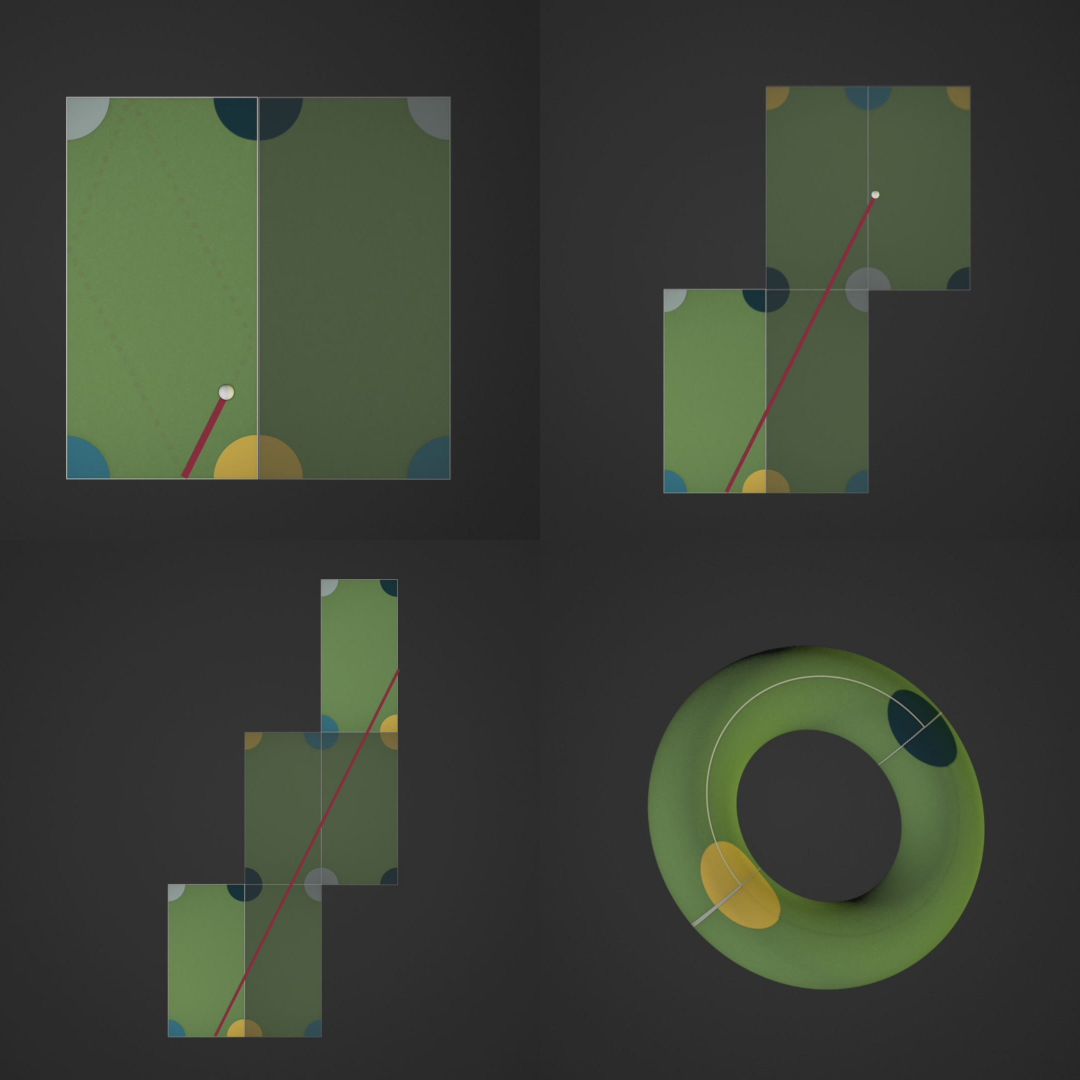
\includegraphics[width=0.75\textwidth,height=\textheight]{img/unfold-in-four-images.png}
\caption{Dépliage d'une trajectoire de billard sur une table
rectangulaire}
\end{figure}
\end{frame}

\begin{frame}{Exemple: la surface en L}
\protect\hypertarget{exemple-la-surface-en-l}{}
\begin{figure}
\centering
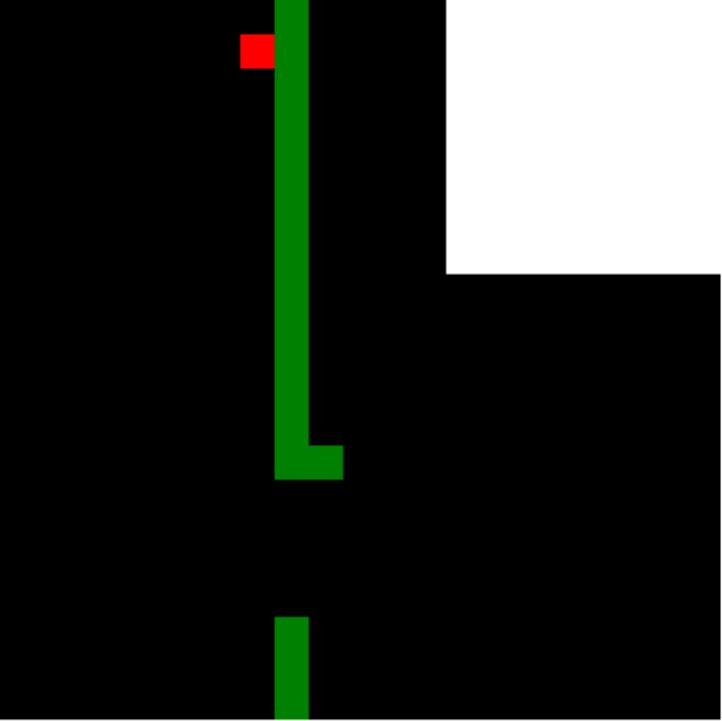
\includegraphics[width=0.6\textwidth,height=\textheight]{img/snake-L-1.png}
\caption{\href{http://albamath.com/snake-L}{Jeu du serpent sur un L},
par MS}
\end{figure}
\end{frame}

\begin{frame}{Surfaces de translation et billards «infinis»}
\protect\hypertarget{surfaces-de-translation-et-billards-infinis}{}
Le dépliage d'un billard irrationnel est une surface de genre infini.

\begin{figure}
\centering
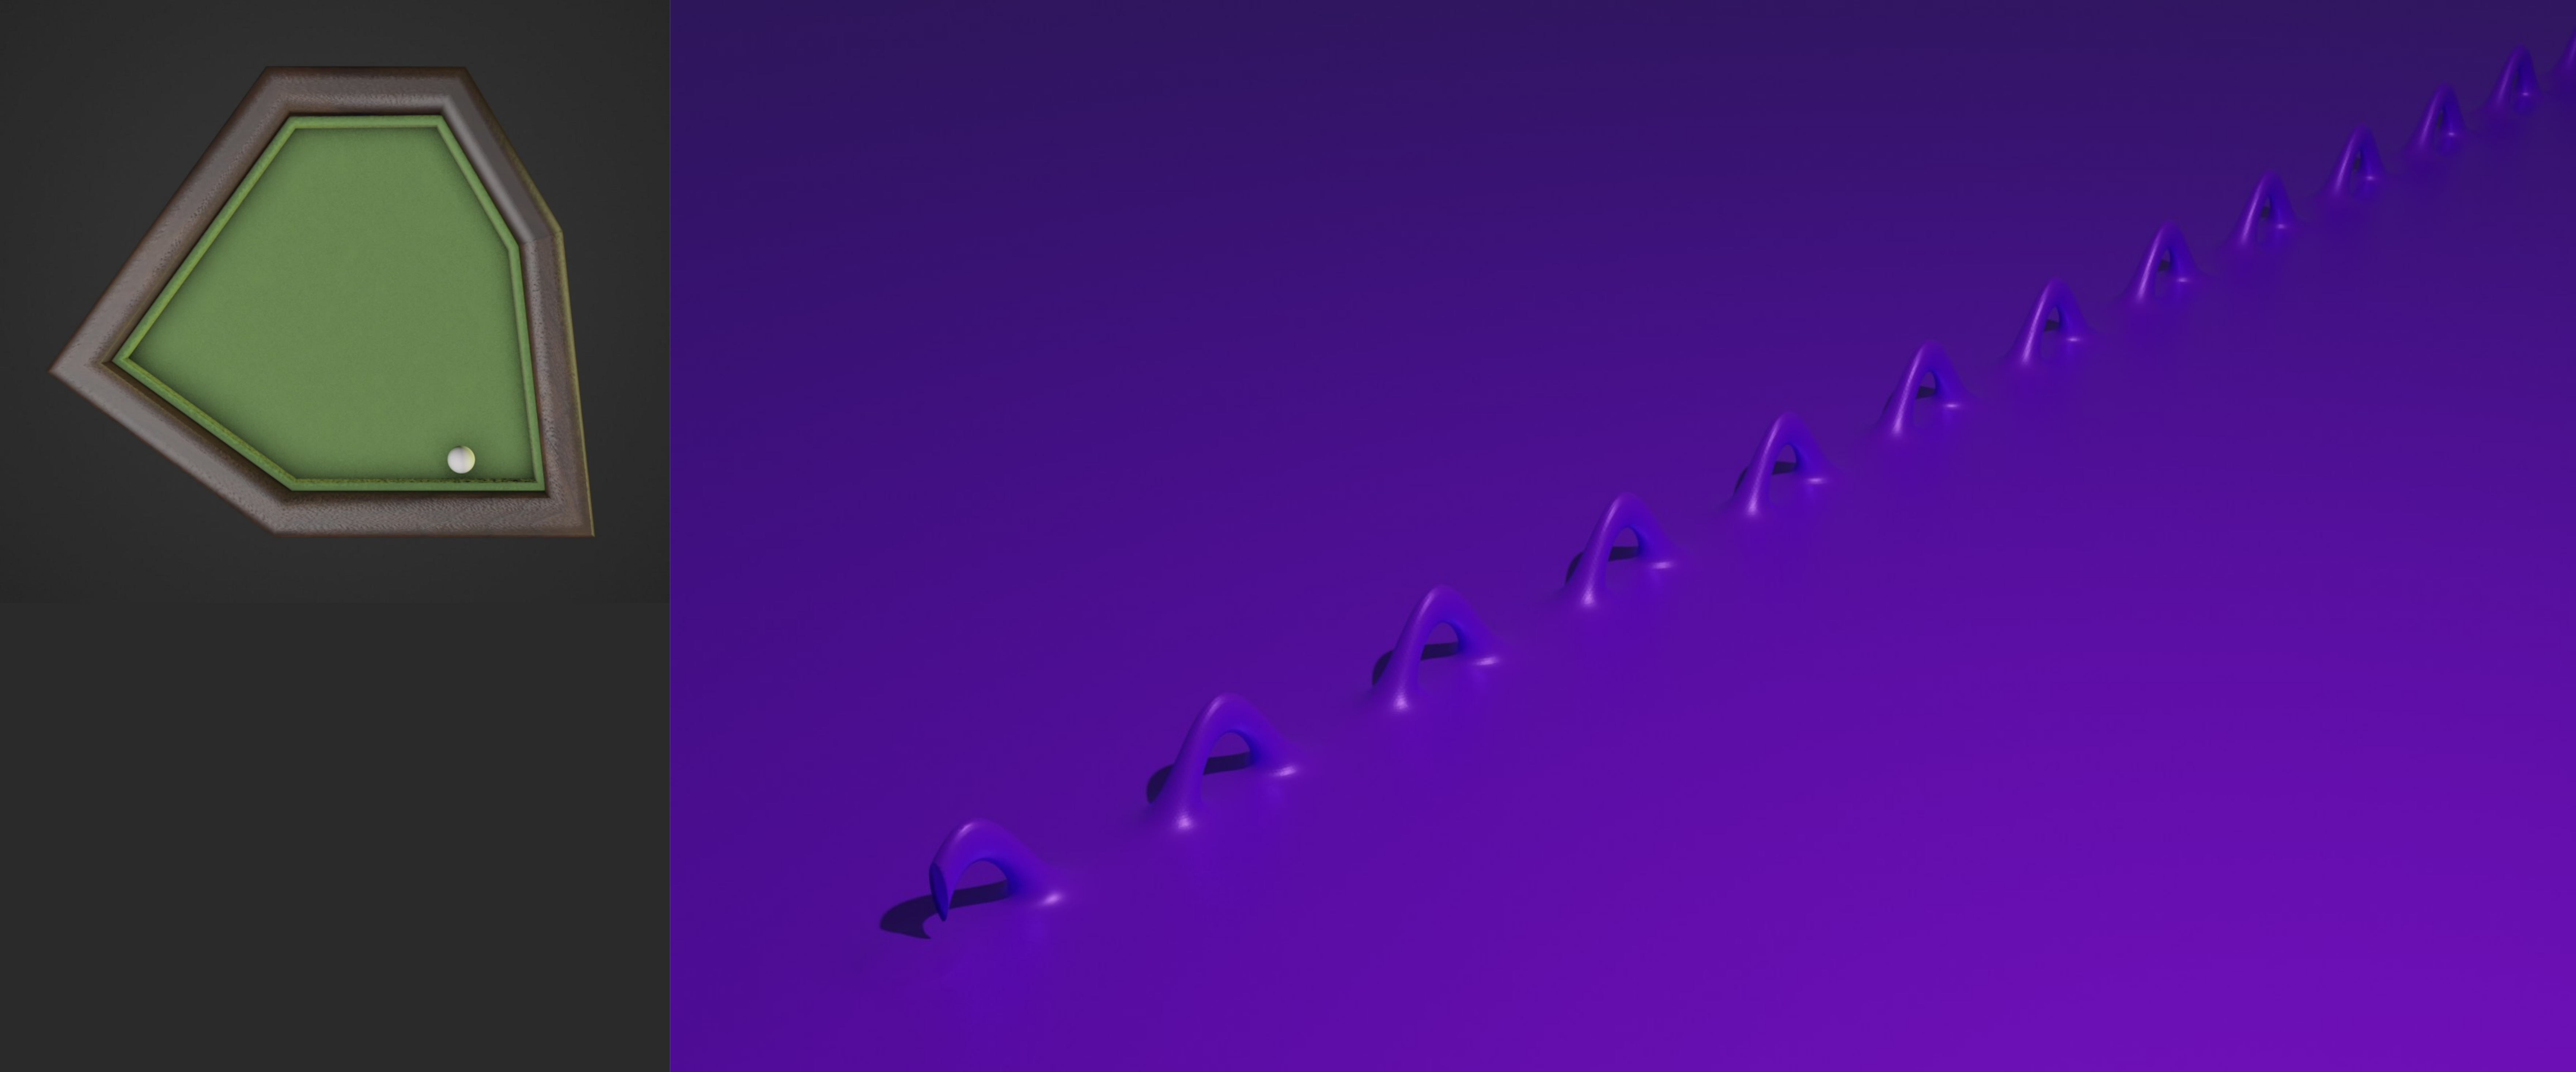
\includegraphics[width=1\textwidth,height=\textheight]{img/billiard-with-loch-ness.png}
\caption{Billard irrationnel par Hale, monstre du Loch Ness par MS.}
\end{figure}
\end{frame}

\begin{frame}{Surfaces de translation et billards «infinis»}
\protect\hypertarget{surfaces-de-translation-et-billards-infinis-1}{}
\begin{figure}
\centering
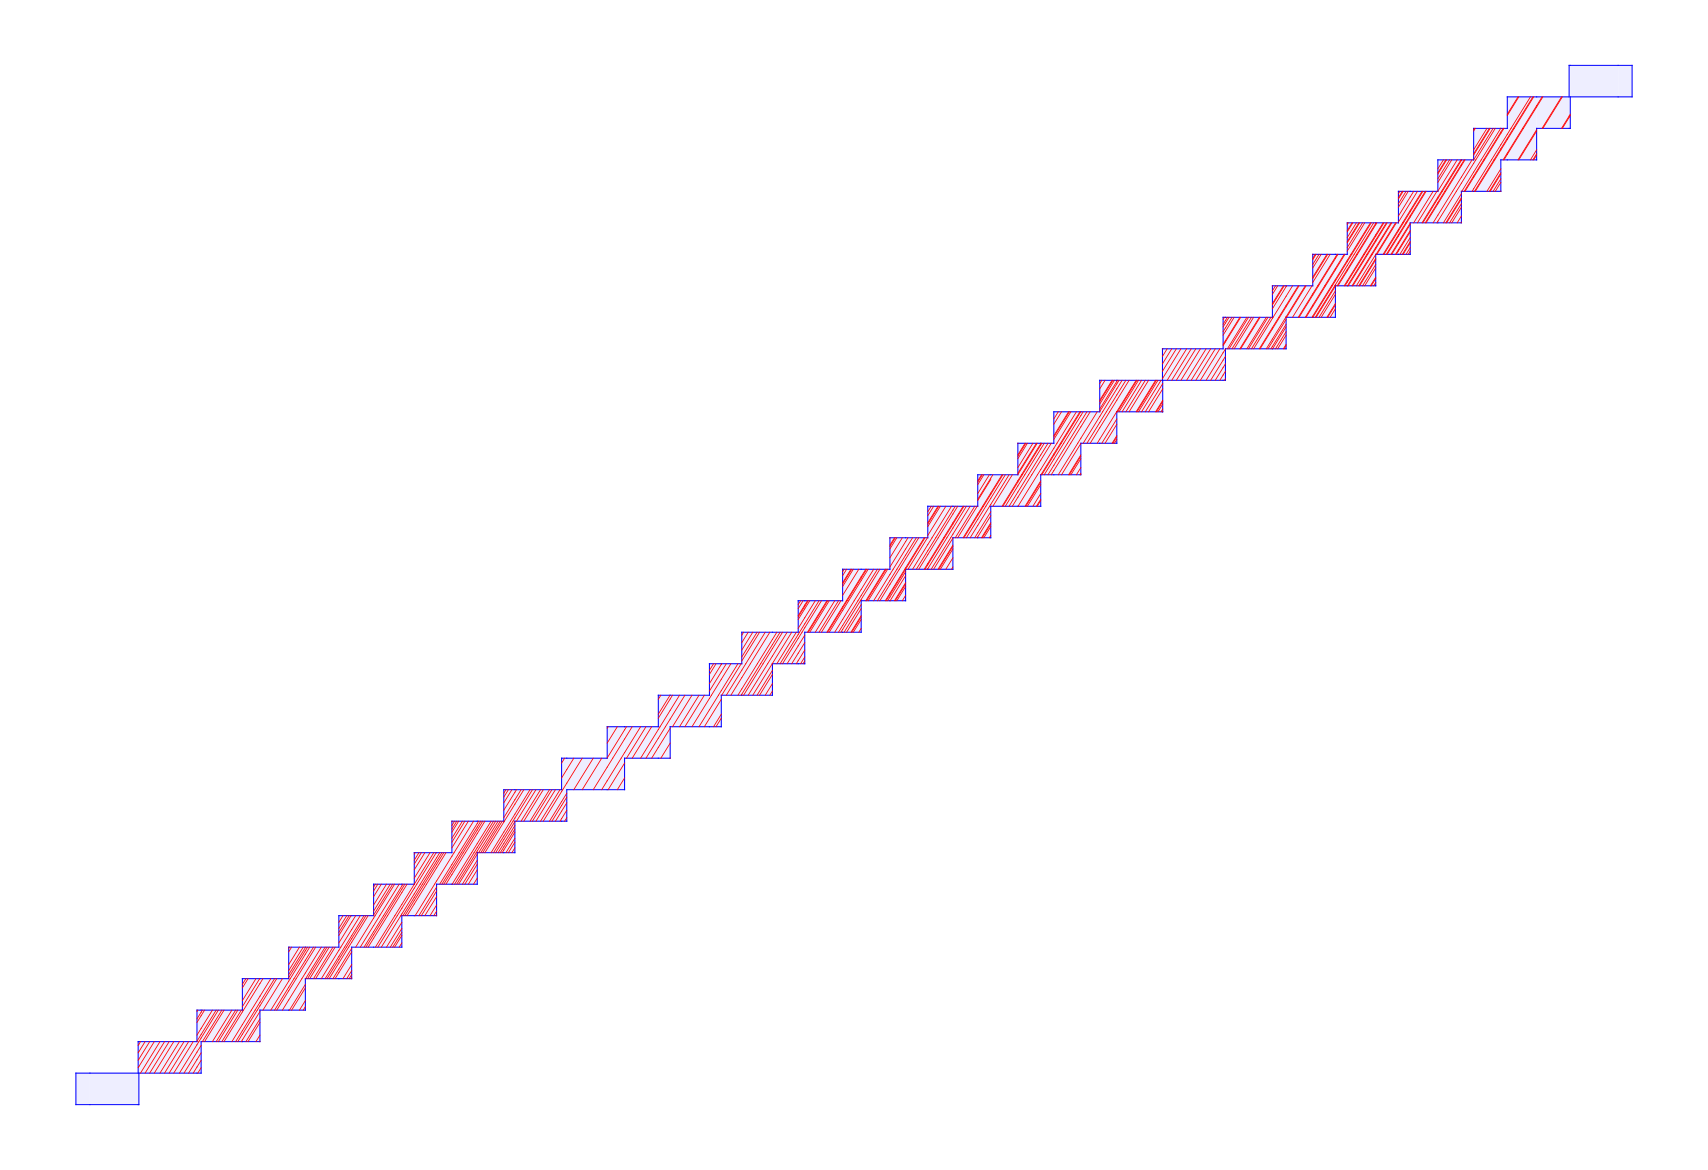
\includegraphics[width=\textwidth,height=4.6875in]{img/escalier-recollement-variable.png}
\caption{Escalier à recollement variable}
\end{figure}
\end{frame}

\begin{frame}{Surfaces de translation et billards «infinis»}
\protect\hypertarget{surfaces-de-translation-et-billards-infinis-2}{}
\begin{figure}
\centering
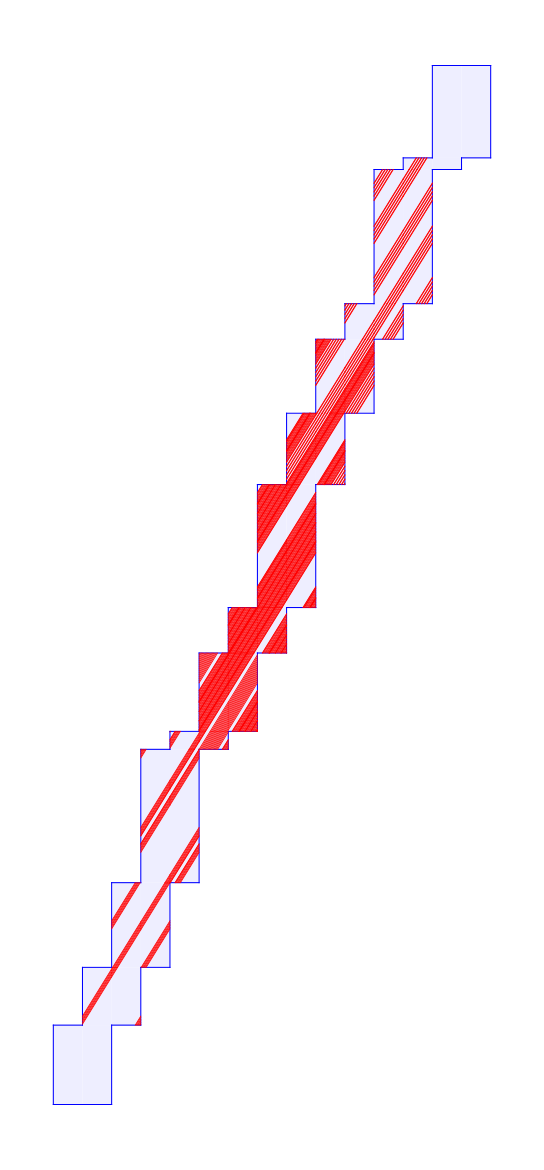
\includegraphics[width=\textwidth,height=2.91667in]{img/escalier-hauteur-variable-sage.png}
\caption{Escalier à hauteur variable}
\end{figure}
\end{frame}

\begin{frame}{Surfaces de translation et billards «infinis»}
\protect\hypertarget{surfaces-de-translation-et-billards-infinis-3}{}
\begin{figure}
\centering
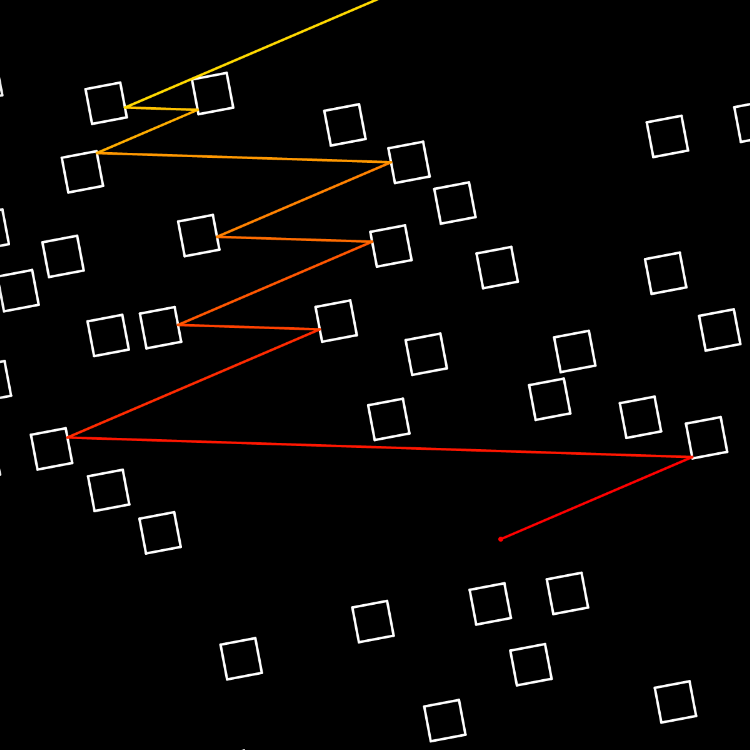
\includegraphics[width=0.6\textwidth,height=\textheight]{img/wind-tree.png}
\caption{Dynamique du wind tree,
\href{https://rantonse.no/demos/MirrorRoom/}{par Antonsen}}
\end{figure}
\end{frame}

\begin{frame}{Ma thèse sous la direction de J.-C. Yoccoz}
\protect\hypertarget{ma-thuxe8se-sous-la-direction-de-j.-c.-yoccoz}{}
J'ai soutenu en 2014 à Orsay une thèse de doctorat intitulée

\emph{Étude d'une famille de transformations\\
préservant la mesure de \(ℤ × 𝕋\).}

sous la direction de Jean-Christophe Yoccoz (Collège de France).

Mes résultats sur \(ℤ × 𝕋\) peuvent s'exprimer en termes de dynamique
des escaliers infinis.

\textbf{Thm} (2014) Si l'on fixe une direction dans le plan alors la
dynamique d'un escalier générique dans cette direction est conservative,
minimale et ergodique.
\end{frame}

\begin{frame}{Mes travaux avec Serge Troubetzkoy}
\protect\hypertarget{mes-travaux-avec-serge-troubetzkoy}{}
Nous poussons beaucoup plus loin les thèmes de ma thèse.

\textbf{Thm} (2015) Génériquement, la dynamique du wind-tree est
minimale dans un large ensemble de directions.

\textbf{Thm} (2016) Génériquement, la dynamique du wind-tree dans
presque toute direction est ergodique.

\textbf{Thm} (2016) La dynamique d'un billard VH est faiblement
mélangeante dans un large ensemble de directions.

\textbf{Thm} (2017) Génériquement, la dynamique du wind-tree est
d'indice ergodique infini dans un large ensemble de directions.

\textbf{Thm} (2019) Génériquement, la dynamique des surfaces en escalier
est uniquement ergodique dans un large ensemble de directions.

\textbf{Thm} (2019) Génériquement, la dynamique du wind-tree est
uniquement ergodique dans un large ensemble de directions.
\end{frame}

\begin{frame}{Publications --- disponibles sur HAL}
\protect\hypertarget{publications-disponibles-sur-hal}{}
Alba Málaga Sabogal, Serge Troubetzkoy (2016)\\
Minimality of the Ehrenfest wind-tree model\\
\emph{Journal of modern dynamics} 10 (209--228)

Alba Málaga Sabogal, Serge Troubetzkoy (2016)\\
Ergodicity of the Ehrenfest wind--tree model\\
\emph{Comptes rendus mathématique} 354:10 (1032--1036)

Alba Málaga Sabogal, Serge Troubetzkoy (2017)\\
Weakly mixing polygonal billiards\\
\emph{Bull. London Math. Soc.} 49 (141--147)

Alba Málaga Sabogal, Serge Troubetzkoy (2018)\\
Infinite ergodic index of the Ehrenfest wind-tree model\\
\emph{Commun. Math. Phys.} 358 (995--1006)

Alba Málaga Sabogal, Serge Troubetzkoy (2019)\\
Unique ergodicity of infinite area translation surfaces\\
\emph{Prépublication} (25 p.)
\end{frame}

\hypertarget{enseignements}{%
\section{Enseignements}\label{enseignements}}

\begin{frame}{Expérience d'enseignement}
\protect\hypertarget{expuxe9rience-denseignement}{}
\begin{longtable}[]{@{}rlll@{}}
\toprule
& Lieu & & Quelques cours\tabularnewline
\midrule
\endhead
2018-2019 & Paris-Saclay, 60h & info &

\includegraphics[width=0.075\textwidth,height=\textheight]{img/logo-upsaclay.png}\tabularnewline
2016-2017 & Paris 8, 192h & info &

\includegraphics[width=0.075\textwidth,height=\textheight]{img/logo-up8.png}\tabularnewline
& & L2 MIASHS & Math. numériques\tabularnewline
2015-2016 & Paris-Sud, 192h & math &

\includegraphics[width=0.075\textwidth,height=\textheight]{img/logo-upsaclay.png}\tabularnewline
& & L3 BS, C & Équa. diff.\tabularnewline
& & L1 MPI & Algèbre linéaire\tabularnewline
& & PCSO & Géométrie, Analyse\tabularnewline
2014 & Paris-Sud, 96h & math &

\includegraphics[width=0.075\textwidth,height=\textheight]{img/logo-upsud.png}\tabularnewline
& & L2 BC & Équa. diff.\tabularnewline
2008 & UNI Lima, 192h & math &

\includegraphics[width=0.075\textwidth,height=\textheight]{img/logo-uni.png}\tabularnewline
& & L2 M & Algèbre linéaire\tabularnewline
& & L1 MPC & Calcul vectoriel\tabularnewline
\bottomrule
\end{longtable}

\textbf{\textgreater600h} dont 192h responsable de cours
\end{frame}

\begin{frame}{Cours, cours intégrés, TD}
\protect\hypertarget{cours-cours-intuxe9gruxe9s-td}{}
Enseignements déjà dispensés:

\begin{itemize}
\tightlist
\item
  Équations différentielles
\item
  Mathématiques numériques avec Python
\item
  Calculus
\item
  Analyse
\item
  Calcul formel avec SageMath
\item
  Structures algébriques
\item
  Gestion de contenu avec Wordpress
\item
  Algèbre linéaire
\item
  Calcul vectoriel
\item
  Calcul intégral
\item
  Programmation orientée objet avec Java
\item
  Introduction à l'informatique avec C++
\end{itemize}
\end{frame}

\begin{frame}{Facultés d'adaptation}
\protect\hypertarget{facultuxe9s-dadaptation}{}
\begin{itemize}
\item
  Programme du lycée très différent du mien

  \begin{itemize}
  \tightlist
  \item
    j'ai étudié les programmes (EduScol)
  \end{itemize}
\item
  Cours de maths numériques sans ordinateurs

  \begin{itemize}
  \tightlist
  \item
    Python sur smartphone (console Android)
  \end{itemize}
\item
  Étudiants d'origines diverses

  \begin{itemize}
  \tightlist
  \item
    je peux enseigner en français, anglais, espagnol, polonais
  \end{itemize}
\item
  Souci d'accessibilité

  \begin{itemize}
  \tightlist
  \item
    supports accessibles pour étudiants aveugles
  \end{itemize}
\end{itemize}
\end{frame}

\begin{frame}{Cours de mathématiques à la FSEG à Créteil}
\protect\hypertarget{cours-de-mathuxe9matiques-uxe0-la-fseg-uxe0-cruxe9teil}{}
Bases mathématiques de modélisation économique et de gestion,\\
en licence. Dans les maquettes actuelles:

\begin{longtable}[]{@{}ll@{}}
\toprule
Année & Intitulé du cours\tabularnewline
\midrule
\endhead
Parcours amenagé & Mathématiques\tabularnewline
& Statistiques descriptives I\tabularnewline
L1 & Mathématiques\tabularnewline
& Statistiques et outils informatiques I\tabularnewline
Passerelle & Outils mathématiques\tabularnewline
& Statistiques descriptives sur Excel\tabularnewline
L2 & Mathématiques\tabularnewline
& \textbf{Probabilités, estimation et tests}\tabularnewline
L3 & \textbf{Mathématiques des systèmes dynamiques}\tabularnewline
& Processus stochastiques en finance\tabularnewline
& Optimisation dynamique\tabularnewline
\bottomrule
\end{longtable}

Master: science des données, apprentissage automatique, \ldots{}
\end{frame}

\begin{frame}{Future adaptation à la FSEG à Créteil}
\protect\hypertarget{future-adaptation-uxe0-la-fseg-uxe0-cruxe9teil}{}
\begin{itemize}
\tightlist
\item
  je connais Python et R
\item
  j'ai enseigné les équations différentielles dans divers parcours
\item
  j'ai fait de l'apprentissage machine
\item
  je suis prête à apprendre SAS, EViews, Stata
\item
  intérêt personnel pour l'économie\\
  lectures: Jean Tirole, Esther Duflo, Joseph Stiglitz, \ldots{}
\item
  apprendre tout au long de la vie, c'est ma devise
\item
  idées de projets avec des étudiants en économie
\end{itemize}
\end{frame}

\begin{frame}{Idées de projets avec des étudiants en économie}
\protect\hypertarget{iduxe9es-de-projets-avec-des-uxe9tudiants-en-uxe9conomie}{}
\begin{itemize}
\tightlist
\item
  Grands perdants du Covid-19: exodes urbains-ruraux en 2020
\item
  Pointeuses numériques et revenu des travailleurs indépendants
\item
  Recensements de population universels vs randomisés
\item
  Résultats Pisa et politiques éducatives des pays de l'OCDE
\item
  Gratuité des transports et usage de la voiture
\item
  Répartition des revenus: outils d'analyse,\\
  vision synchronique et diachronique
\item
  Les systèmes d'imposition et leur évolution
\item
  Croissance économique: vision à court terme et long terme
\item
  Le coût de la santé
\item
  Le financement des retraites
\end{itemize}
\end{frame}

\hypertarget{autres-activituxe9s}{%
\section{Autres activités}\label{autres-activituxe9s}}

\begin{frame}{Autres activités}
\begin{figure}
\centering
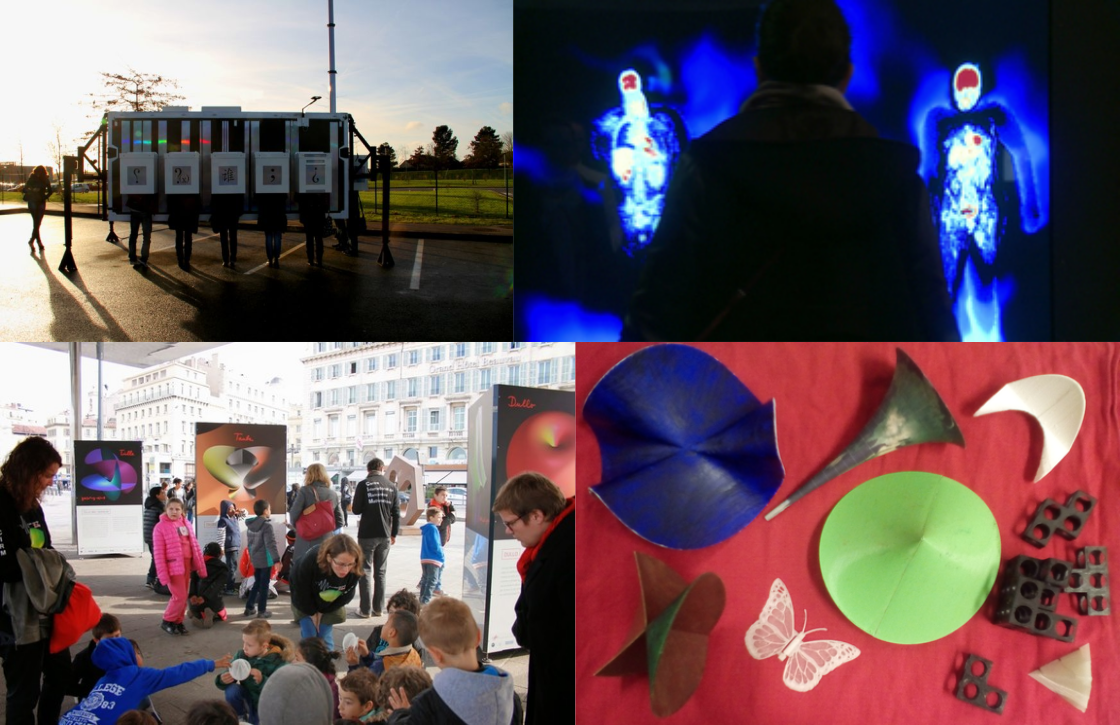
\includegraphics[width=0.8\textwidth,height=\textheight]{img/quatre-images-mediation.png}
\caption{Médiation scientifique}
\end{figure}

\(\sim\) 30 expositions, forums, salons, exposés, \ldots{}
\end{frame}

\hypertarget{conclusion}{%
\section{Conclusion}\label{conclusion}}

\begin{frame}{Pour finir\ldots{}}
\protect\hypertarget{pour-finir}{}
\begin{longtable}[]{@{}lll@{}}
\toprule
\endhead
\begin{minipage}[t]{0.32\columnwidth}\raggedright
parcours polyvalent\strut
\end{minipage} & \begin{minipage}[t]{0.29\columnwidth}\raggedright
un vrai souci de l'accessibilité\strut
\end{minipage} & \begin{minipage}[t]{0.30\columnwidth}\raggedright
fibre «maker»\strut
\end{minipage}\tabularnewline
\begin{minipage}[t]{0.32\columnwidth}\raggedright
intérêt en médiation scientifique\strut
\end{minipage} & \begin{minipage}[t]{0.29\columnwidth}\raggedright
enseignement dans le respect\strut
\end{minipage} & \begin{minipage}[t]{0.30\columnwidth}\raggedright
continuité dans la recherche\strut
\end{minipage}\tabularnewline
\bottomrule
\end{longtable}

J'ai à cœur de m'intégrer dans la recherche au LAMA et dans
l'enseignement à la FSEG.

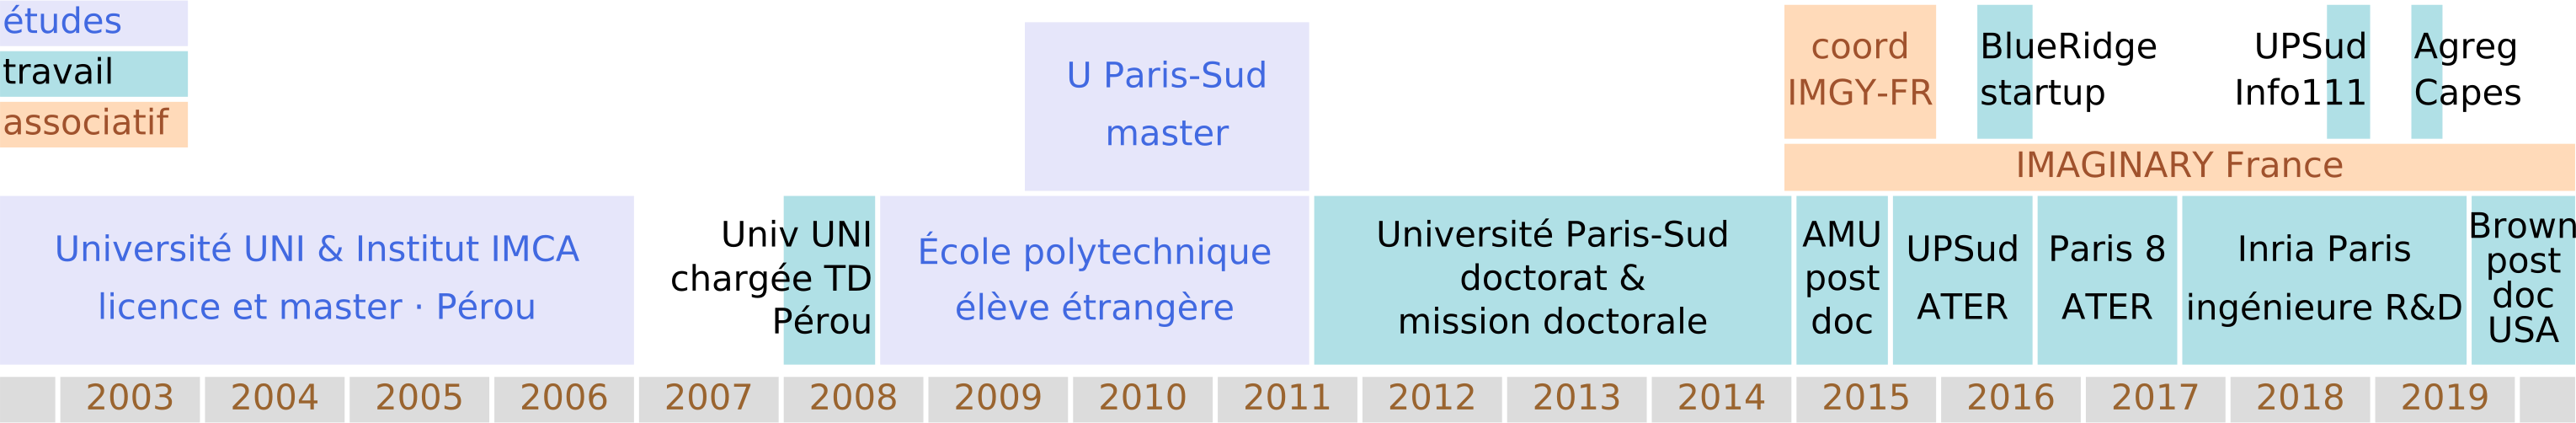
\includegraphics[width=1\textwidth,height=\textheight]{img/alba-timeline.png}
\end{frame}

\end{document}
